\documentclass[14pt,a4paper]{extarticle}

\usepackage[utf8]{inputenc}
\usepackage[T2A]{fontenc}
\usepackage{amssymb,amsmath,mathrsfs,amsthm}
\usepackage[russian]{babel}
\usepackage{graphicx}
\usepackage[footnotesize]{caption2}
\usepackage{indentfirst}
\usepackage{multicol}
\usepackage{listings}
\usepackage{float}
\usepackage{url}
\usepackage{amsmath}

\usepackage{enumitem}

%\usepackage[ruled,section]{algorithm}
%\usepackage[noend]{algorithmic}
%\usepackage[all]{xy}
\usepackage{booktabs}
\usepackage{graphicx}
\usepackage[table,xcdraw]{xcolor}
\usepackage{tcolorbox}

%Библиотека для блок-схем
\usepackage{tikz}
\usetikzlibrary{shapes,arrows}

% Параметры страницы
\textheight=24cm
\textwidth=16cm
\oddsidemargin=5mm
\evensidemargin=-5mm
\marginparwidth=36pt
\topmargin=-1cm
\footnotesep=3ex
%\flushbottom
\raggedbottom
\tolerance 3000
% подавить эффект "висячих стpок"
\clubpenalty=10000
\widowpenalty=10000
%\renewcommand{\baselinestretch}{1.1}
\renewcommand{\baselinestretch}{1.5} %для печати с большим интервалом

\newcommand{\angstrom}{\mbox{\normalfont\AA}}

\newtheorem{definition}{Определение} % задаём выводимое слово (для определений)
\newtheorem{example}{Замечание} % задаём выводимое слово (для определений)
\newtheorem{theorem}{Теорема} % задаём выводимое слово (для определений)
\newtheorem{proposition}{Утверждение} % задаём выводимое слово (для определений)
\newtheorem{construction}{Конструкция} % задаём выводимое слово (для определений)

\DeclareMathOperator*{\sgn}{sgn}
\DeclareMathOperator*{\var}{var}
\DeclareMathOperator*{\cov}{cov}
\DeclareMathOperator*{\law}{Law}

\newcommand{\1}{\mathbbm{1}}
\newcommand{\R}{\mathbb{R}}
\newcommand{\N}{\mathbb{N}}
\newcommand{\Z}{\mathbb{Z}}
\renewcommand{\P}{\mathbb{P}}
\newcommand{\E}{\mathbb{E}}

\newcommand{\independent}{\perp\!\!\!\!\perp}

\newcommand\cA{{\cal A}}
\newcommand\cE{{\cal E}}
\newcommand\cC{{\cal C}}
\newcommand\cF{{\cal F}}
\newcommand\cG{{\cal G}}
\newcommand\cK{{\cal K}}
\newcommand\cL{{\cal L}}
\newcommand\cB{{\cal B}}
\newcommand\cN{{\cal N}}
\newcommand\cM{{\cal M}}
\newcommand\cX{{\cal X}}
\newcommand\cD{{\cal D}}
\newcommand\cR{{\cal R}}
\newcommand\cP{{\cal P}}
\newcommand\cQ{{\cal Q}}
\newcommand\cS{{\cal S}}
\newcommand\cT{{\cal T}}
\newcommand\cV{{\cal V}}
\newcommand\cZ{{\cal Z}}

\newcommand{\textProposition}    {Предложение}
\newcommand{\textTask}    {Задача}

\begin{document}

\begin{center}
    {Всеволод Заостровский, 409 группа}\\
    {\bfseries Отчёт по задаче ''Решение уравнения типа теплопроводности с коэффициентами в дивергенции''.\\}
    \vspace{1cm}
\end{center}

\tableofcontents

\section{Постановка задачи.} \label{diffeq1}
\subsection{Одномерный Лаплас}
Необходимо решить уравнение:
\begin{equation*} 
    u_t(t, x) = \operatorname{div} (k(x) \operatorname{grad} u(t, x)).
\end{equation*}
Будем считать, что $0 \leq t,x \leq 1$. В моём варианте, краевые условия:
\begin{align*} 
    &u(t, x) \big| _{x \in \partial \Omega} = 0, \quad \Omega = [0,1]. \\
    &u(0, x) = u^0(x), \quad x \in \Omega. 
\end{align*}

\subsection{Двумерный Лаплас}
Необходимо решить уравнение:
\begin{equation*} 
    u_t(t, x, y) = \operatorname{div} (k(x, y) \operatorname{grad} u(t, x, y)).
\end{equation*}
Будем считать, что $0 \leq t,x,y \leq 1$. В моём варианте, краевые условия:
\begin{align*} 
    &u(t, x, y) \big| _{(x ,y) \in \partial \Omega} = 0, \quad \Omega = [0,1] \times [0,1]. \\
    &u(0, x, y) = u^0(x, y), \quad (x, y) \in \Omega. 
\end{align*}

\section{Алгоритм решения одномерной схемы.}
\subsection{Дискретизация}
Уравнение будем приближать посредством следующей схемы:
\begin{align*}
    &\frac{u^{n+1}_i - u^n_i}{\tau} = \frac{k(x_{i + \frac{1}{2}}) \frac{u^{n+1}_{i+1} - u^{n+1}_{i}}{h} - k(x_{i- \frac{1}{2}}) \frac{u^{n+1}_{i} - u^{n+1}_{i-1}}{h}}{h}.
\end{align*}
Краевые условия:
\begin{align*} 
    &u(t, x) \big| _{x \in \partial \Omega} = 0, \quad \Omega = [0,1]. \\
    &u(0, x) = u^0(x), \quad x \in \Omega. 
\end{align*}
\subsection{Общий вид матрицы уравнения.}
Преобразуем схему:
\begin{align*}
    u^{n+1}_i - u^n_i = \tau k(x_{i + \frac{1}{2}}) \frac{u^{n+1}_{i+1} - u^{n+1}_{i}}{h^2} - \tau k(x_{i- \frac{1}{2}}) \frac{u^{n+1}_{i} - u^{n+1}_{i-1}}{h^2}.\\
    u^{n+1}_i - u^n_i = 
    \tau k(x_{i + \frac{1}{2}}) \frac{u^{n+1}_{i+1} }{h^2} 
    - u^{n+1}_i \frac{\tau}{h^2} (k(x_{i + \frac{1}{2}}) + k(x_{i - \frac{1}{2}})) 
    + \tau k(x_{i- \frac{1}{2}}) \frac{u^{n+1}_{i-1}}{h^2}. 
\end{align*}
Таким образом, получим:
\begin{equation}
    - u^{n+1}_{i+1} k(x_{i + \frac{1}{2}}) \frac{\tau}{h^2} +
    u^{n+1}_i\left(1 + \frac{\tau}{h^2} (k(x_{i + \frac{1}{2}}) + k(x_{i - \frac{1}{2}}))\right) - u^{n+1}_{i-1} k(x_{i- \frac{1}{2}}) \frac{ \tau}{h^2} = u^n_i.
\end{equation}
Матрица примет вид: \\
$$A = \begin{pmatrix}
    c   & b_+ & 0     & 0   & 0   & \ldots & 0 \\
    b_- & c   & b_+   & 0   & 0   & \ldots & 0 \\
    0   & b_- & c     & b_+ & 0   & \ldots & 0 \\
    0   & 0   & b_-   & c   & b_+ & \ldots & 0 \\
    \ldots & \ldots & \ldots & \ldots & \ldots & \ldots & \ldots \\
    0   & 0   & 0    & \ldots & b_- & c & b_+ \\
    0   & 0   & 0     & \ldots & 0 & b_- & c \\
\end{pmatrix}, \text{где}
\left\{\begin{array}{l}
 c = 1 + \frac{\tau}{h^2} (k(x_{i + \frac{1}{2}}) + k(x_{i - \frac{1}{2}})), \\
 b_+ = -k(x_{i + \frac{1}{2}}) \frac{\tau}{h^2}, \\
 b_- = -k(x_{i - \frac{1}{2}}) \frac{\tau}{h^2}.
\end{array}\right. 
$$
\subsection{Решение схемы.}
Итоговый вид интересующей нас системы:
\begin{align*}
    A u^{n+1} = u^n, \quad u^n := (u^n_0, u^n_1, \ldots u^n_{N_X}).
\end{align*}
Как видно, эту системы легко решить методом прогонки: двигаясь от 0-го слоя к $N$-му. Несколько сложнее дела обстоят с двумерной схемой, которая описана ниже.

\section{Алгоритм решения двумерной схемы.}
\subsection{Дискретизация.}
Уравнение будем приближать посредством следующей схемы:
\begin{align*}
    \frac{u^{n+1}_i - u^n_i}{\tau} &= \frac{k(x_{i + \frac{1}{2}, j}) \frac{u^{n+1}_{i+1, j} - u^{n+1}_{i, j}}{h_X} - k(x_{i- \frac{1}{2}, j}) \frac{u^{n+1}_{i, j} - u^{n+1}_{i-1, j}}{h_X}}{h_X} + \\
    &+  \frac{k(x_{i, j + \frac{1}{2}}) \frac{u^{n+1}_{i, j+1} - u^{n+1}_{i, j}}{h_Y} - k(x_{i, j- \frac{1}{2}}) \frac{u^{n+1}_{i, j} - u^{n+1}_{i, j-1}}{h_Y}}{h_Y}.
\end{align*}
Краевые условия:
\begin{align*} 
    &u(t, x, y) \big| _{(x, y) \in \partial \Omega} = 0, \quad \Omega = [0,1] \times [0, 1]. \\
    &u(0, x, y) = u^0(x, y), \quad x \in \Omega. 
\end{align*}
\subsection{Общий вид матрицы уравнения.} \label{generalmatrix2d}
Для придания выкладкам хоть сколько-нибудь приемлемого вида, здесь и далее считаем $h_X = h_Y = h = \frac{1}{N_X - 1}, \quad N_X = N_Y$.
Пользуясь вычислениями из предыдущего раздела, получим:
\begin{align*}
    u^{n+1}_{i, j} - u^n_{i, j} = \tau k(x_{i + \frac{1}{2}}, y_j) \frac{u^{n+1}_{i+1, j} - u^{n+1}_{i, j}}{h^2} - \tau k(x_{i- \frac{1}{2}}, y_j) \frac{u^{n+1}_{i, j} - u^{n+1}_{i-1, j}}{h^2} + \\
    + \tau k(x_{i, y_{j + \frac{1}{2}}}) \frac{u^{n+1}_{i, j+1} - u^{n+1}_{i, j}}{h^2} - \tau k(x_{i}, y_{j - \frac{1}{2}}) \frac{u^{n+1}_{i, j} - u^{n+1}_{i, j-1}}{h^2}. \\
    u^{n+1}_{i, j} - u^n_{i, j} = - u^{n+1}_{i, j} \frac{\tau}{h^2} \left(k(x_{i + \frac{1}{2}}, y_{j}) + k(x_{i - \frac{1}{2}}, y_{j}) + k(x_{i}, y_{j+ \frac{1}{2}}) + k(x_{i}, y_{j- \frac{1}{2}})\right) +\\
    + \tau k(x_{i + \frac{1}{2}}, y_{j}) \frac{u^{n+1}_{i+1,j} }{h^2} 
    + \tau k(x_{i- \frac{1}{2}}, y_{j}) \frac{u^{n+1}_{i-1, j}}{h^2}
    + \tau k(x_{i}, y_{j+ \frac{1}{2}}) \frac{u^{n+1}_{i,j+1} }{h^2} 
    + \tau k(x_{i}, y_{j- \frac{1}{2}}) \frac{u^{n+1}_{i, j-1}}{h^2}. 
\end{align*}
Итоговая схема выглядит следующим образом:
\begin{align*}
    &u^{n+1}_{i, j}\left(\frac{1}{\tau} + \frac{1}{h^2} \left(k(x_{i + \frac{1}{2}}, y_{j}) + k(x_{i - \frac{1}{2}}, y_{j}) + k(x_{i}, y_{j+ \frac{1}{2}}) + k(x_{i}, y_{j- \frac{1}{2}})\right)\right) -\\
    &+ \frac{1}{h^2} \left[- u^{n+1}_{i+1,j} k(x_{i + \frac{1}{2}}, y_{j}) 
    - u^{n+1}_{i-1, j} k(x_{i- \frac{1}{2}}, y_{j})
    - u^{n+1}_{i,j+1} k(x_{i}, y_{j+ \frac{1}{2}}) 
    - u^{n+1}_{i, j-1} k(x_{i}, y_{j- \frac{1}{2}}) \right]\\ &= \frac{u^n_{i, j}}{\tau}.
\end{align*}
Эту схему можно записать в огромную ( $\R ^{N_X^4}$) разреженную блочную матрицу вида:
$$A = \begin{pmatrix}
    I   & 0   & 0     & 0   & 0   & \ldots & 0 \\
    D_-   & C   & D_+   & 0   & 0   & \ldots & 0 \\
    0   & D_-   & C     & D_+ & 0   & \ldots & 0 \\
    0   & 0   & D_-   & C   & D_+ & \ldots & 0 \\
    \ldots & \ldots & \ldots & \ldots & \ldots & \ldots & \ldots \\
    0   & 0   & 0    & \ldots & D_- & C & D_+ \\
    0   & 0   & 0     & \ldots & 0 & 0 & I \\
\end{pmatrix},
$$
описание блоков:
\begin{enumerate}
    \item[Блок $C$:] $$C = \begin{pmatrix}
    c   & b_+ & 0     & 0   & 0   & \ldots & 0 \\
    b_- & c   & b_+   & 0   & 0   & \ldots & 0 \\
    0   & b_- & c     & b_+ & 0   & \ldots & 0 \\
    0   & 0   & b_-   & c   & b_+ & \ldots & 0 \\
    \ldots & \ldots & \ldots & \ldots & \ldots & \ldots & \ldots \\
    0   & 0   & 0    & \ldots & b_- & c & b_+ \\
    0   & 0   & 0     & \ldots & 0 & b_- & c \\
\end{pmatrix},
$$
в матрице $C$:
$$
\left\{\begin{array}{l}
 c = \frac{1}{\tau} + \frac{1}{h^2} \left(k(x_{i + \frac{1}{2}}, y_{j}) + k(x_{i - \frac{1}{2}}, y_{j}) + k(x_{i}, y_{j+ \frac{1}{2}}) + k(x_{i}, y_{j- \frac{1}{2}})\right), \\
 b_+ = -k(x_{i + \frac{1}{2}}, y_j) \frac{1}{h^2}, \\
 b_- = -k(x_{i - \frac{1}{2}}, y_j) \frac{1}{h^2};
\end{array}\right. 
$$
\item[Блок $I$:] $I$ --- единичная матрица размера $N_X\times N_X$; 
\item[Блок $D_-$:] $D_- = -k(x_{i}, y_{j- \frac{1}{2}}) \frac{\tau}{h^2} I =: d_- I$;
\item[Блок $D_+$:] $D_- = -k(x_{i}, y_{j+ \frac{1}{2}}) \frac{\tau}{h^2} I =: d_+ I$.
\end{enumerate}
Итоговый вид уравнения:
\begin{align*}
    A u^{n+1} = \frac{u^n}{\tau}. 
\end{align*}
По предыдущему слою мы будем находить следующий, начиная с 0-го слоя, который нам дан, по условию. Отметим, что мы хотим построить трёхмерную матрицу $U = (u^n_{i, j})^{0 \leq n \leq N} _{0 \leq i, j \leq N_X}$, но форма записи матрицы $A$ предполагаем, что множество $(u^n_{i, j})^{n=\text{const}} _{0 \leq i, j \leq N_X}$ вытягивается в вектор $u^{n}$:
    \begin{align*}
        u^n = (u^n_{0,0}, u^n_{1,0}, u^n_{2,0}, \ldots u^n_{0, 1}, u^n_{0, 2}, \ldots u^n_{0, N_X}, u^n_{1, N_X}, \ldots u^n_{N_X, N_X})^T
    \end{align*}
\subsection{Решение схемы.}
Для решения этой системы также можно применять прогонку (точнее, её более общую модификацию). Мы применим итеративный алгоритм решения с предобуславливателем, который подробно опишем ниже. Общий вид таких алгоритмов:
\begin{align*}
    B \frac{u^{n+1, p+1} - u^{n+1, p+1}}{\theta} + A u^{n+1, p} = b^n.
\end{align*}
В нашем случае, 
\begin{enumerate}
    \item[$A$] --- матрица, описанная в разделе \ref{generalmatrix2d}. Следует отметить, что эта матрица пятидиагональная, так что, несмотря на то, что формально она принадлежит пространству $\R ^{(N_X+1)^4}$, для её хранения требуется лишь $5 * (N_X+1)^2$ памяти (по массиву для каждой из 5 диагоналей), а умножение матрицы на вектор требует $10 * (N_X+1)^2$ арифметических операций.
    \item[$u^{n, p}$] --- результат после $p$-ой итерации процесса для $n$ слоя ответа. Отметим, что мы считаем $u^{n, 0} = u^n$.
    \item[$\theta$] --- итерационный параметр. Наивысшая (в некотором смысле) скорость сходимости достигается при $\theta = \frac{2}{m + M}$, где $M$ и $m$ --- соответственно, максимальное и минимальное собственные значения матрицы. 
    \item[$B$] --- предобуславливатель, берётся разным для разных задач. Мы рассмотрим $B = A \big|_{k(x_i, y_j) = \frac{k(x_0, y_0)+k(x_{N_X}, y_{N_X})}{2}}$.
\end{enumerate}
Итерироваться мы будем следующим образом:
\begin{enumerate}
    \item Заметим, что:
    \begin{align*}
        B \frac{u^{n+1, p+1} - u^{n+1, p+1}}{\theta} + A u^{n+1, p} 
        = \frac{u^{n}}{\tau}\Leftrightarrow 
        \left\{\begin{array}{l}
            B y^{p+1} = \frac{u^{n}}{\tau} - A u^{n+1, p}, \\
            u^{n+1, p+1} = u^{n+1, p} + \theta y^{p+1}.
        \end{array}\right.
    \end{align*}
    \item За $O(N^2)$ вычислим вектор $b - A x^p$.
    \item С помощью метода Фурье за $O(N^3)$ решим систему $B y^{p+1} = b - A x^p$. Схема при этом принимает вид:
\begin{align*}
    &\frac{u^{n+1}_{i,j}}{k \tau} - 
    \frac{u^{n+1}_{i+1, j} - 2 u^{n+1}_{i, j}- u^{n+1}_{i-1, j}}{h^2} -  
    \frac{u^{n+1}_{i, j+1} - 2 u^{n+1}_{i, j}- u^{n+1}_{i, j-1}}{h^2} =\\&= 
    \underbrace{f(x_i, y_j)}_{= (\frac{u^{n}}{\tau} - A u^{n+1, p})/k\big|_{i,j}} = \frac{u^{n}}{k\tau} - \frac{1}{k} A u^{n+1, p}.
\end{align*}

    \item Следующий вектор в итеративной процедуре вычислим по формуле $x^{k+1} = x^k + \tau y^{k+1}$.
\end{enumerate}
\subsection{Алгоритм для программирования.}
На шаге $n$ нам известны слои вплоть до $u^n$ (слой --- матрица, вытянутая в вектор). $u^0$ задан изначально. 
\begin{enumerate} 
    \item Нужно решить уравнение:
    \begin{align*}
        A u^{n+1} = \frac{u^n}{\tau}.
    \end{align*}
    Для этого:
    \begin{enumerate}
        \item Решаем уравнение 
        \begin{align*}
            B y^{k+1} = \frac{u^{n}}{\tau} - A x^k,
        \end{align*}
        где $B$ --- матрица Фурье с постоянным $k$.
        \item Вычисляем $x^{k+1}=x^k + \theta y^{k+1}$.
        \item Повторяем процедуру пока не увидим сходимость.
    \end{enumerate}
    \item Таким образом, от слоя к слою, восстановим всю матрицу.
\end{enumerate}

\section{Тесты.}
\subsection{Простейший случай ($k = \text{const}$)}
Для простоты сравнения с предыдущим отчетом было рассмотрено $k=1$. В целом, всё аналогично 
предыдущему случаю, поэтому здесь не проводилось более глубоких тестов. На графике \ref{constk} по оси $y$ отложено значение функции, 
по оси $x$ --- порядковый номер тройки точек $(x, y, z)$: вывод задачи представлен в виде 
$$
(x,y,z,\text{численное решение}, \text{аналитическое решение})
$$ 
и, при 
заданном разбиении каждой точки равномерной сетки соответствует натуральное число.  

Отметим, что сходимость итерационного алгоритма в этом случае происходила за одну итерацию, как и должно быть.

\begin{figure}
    \centering
    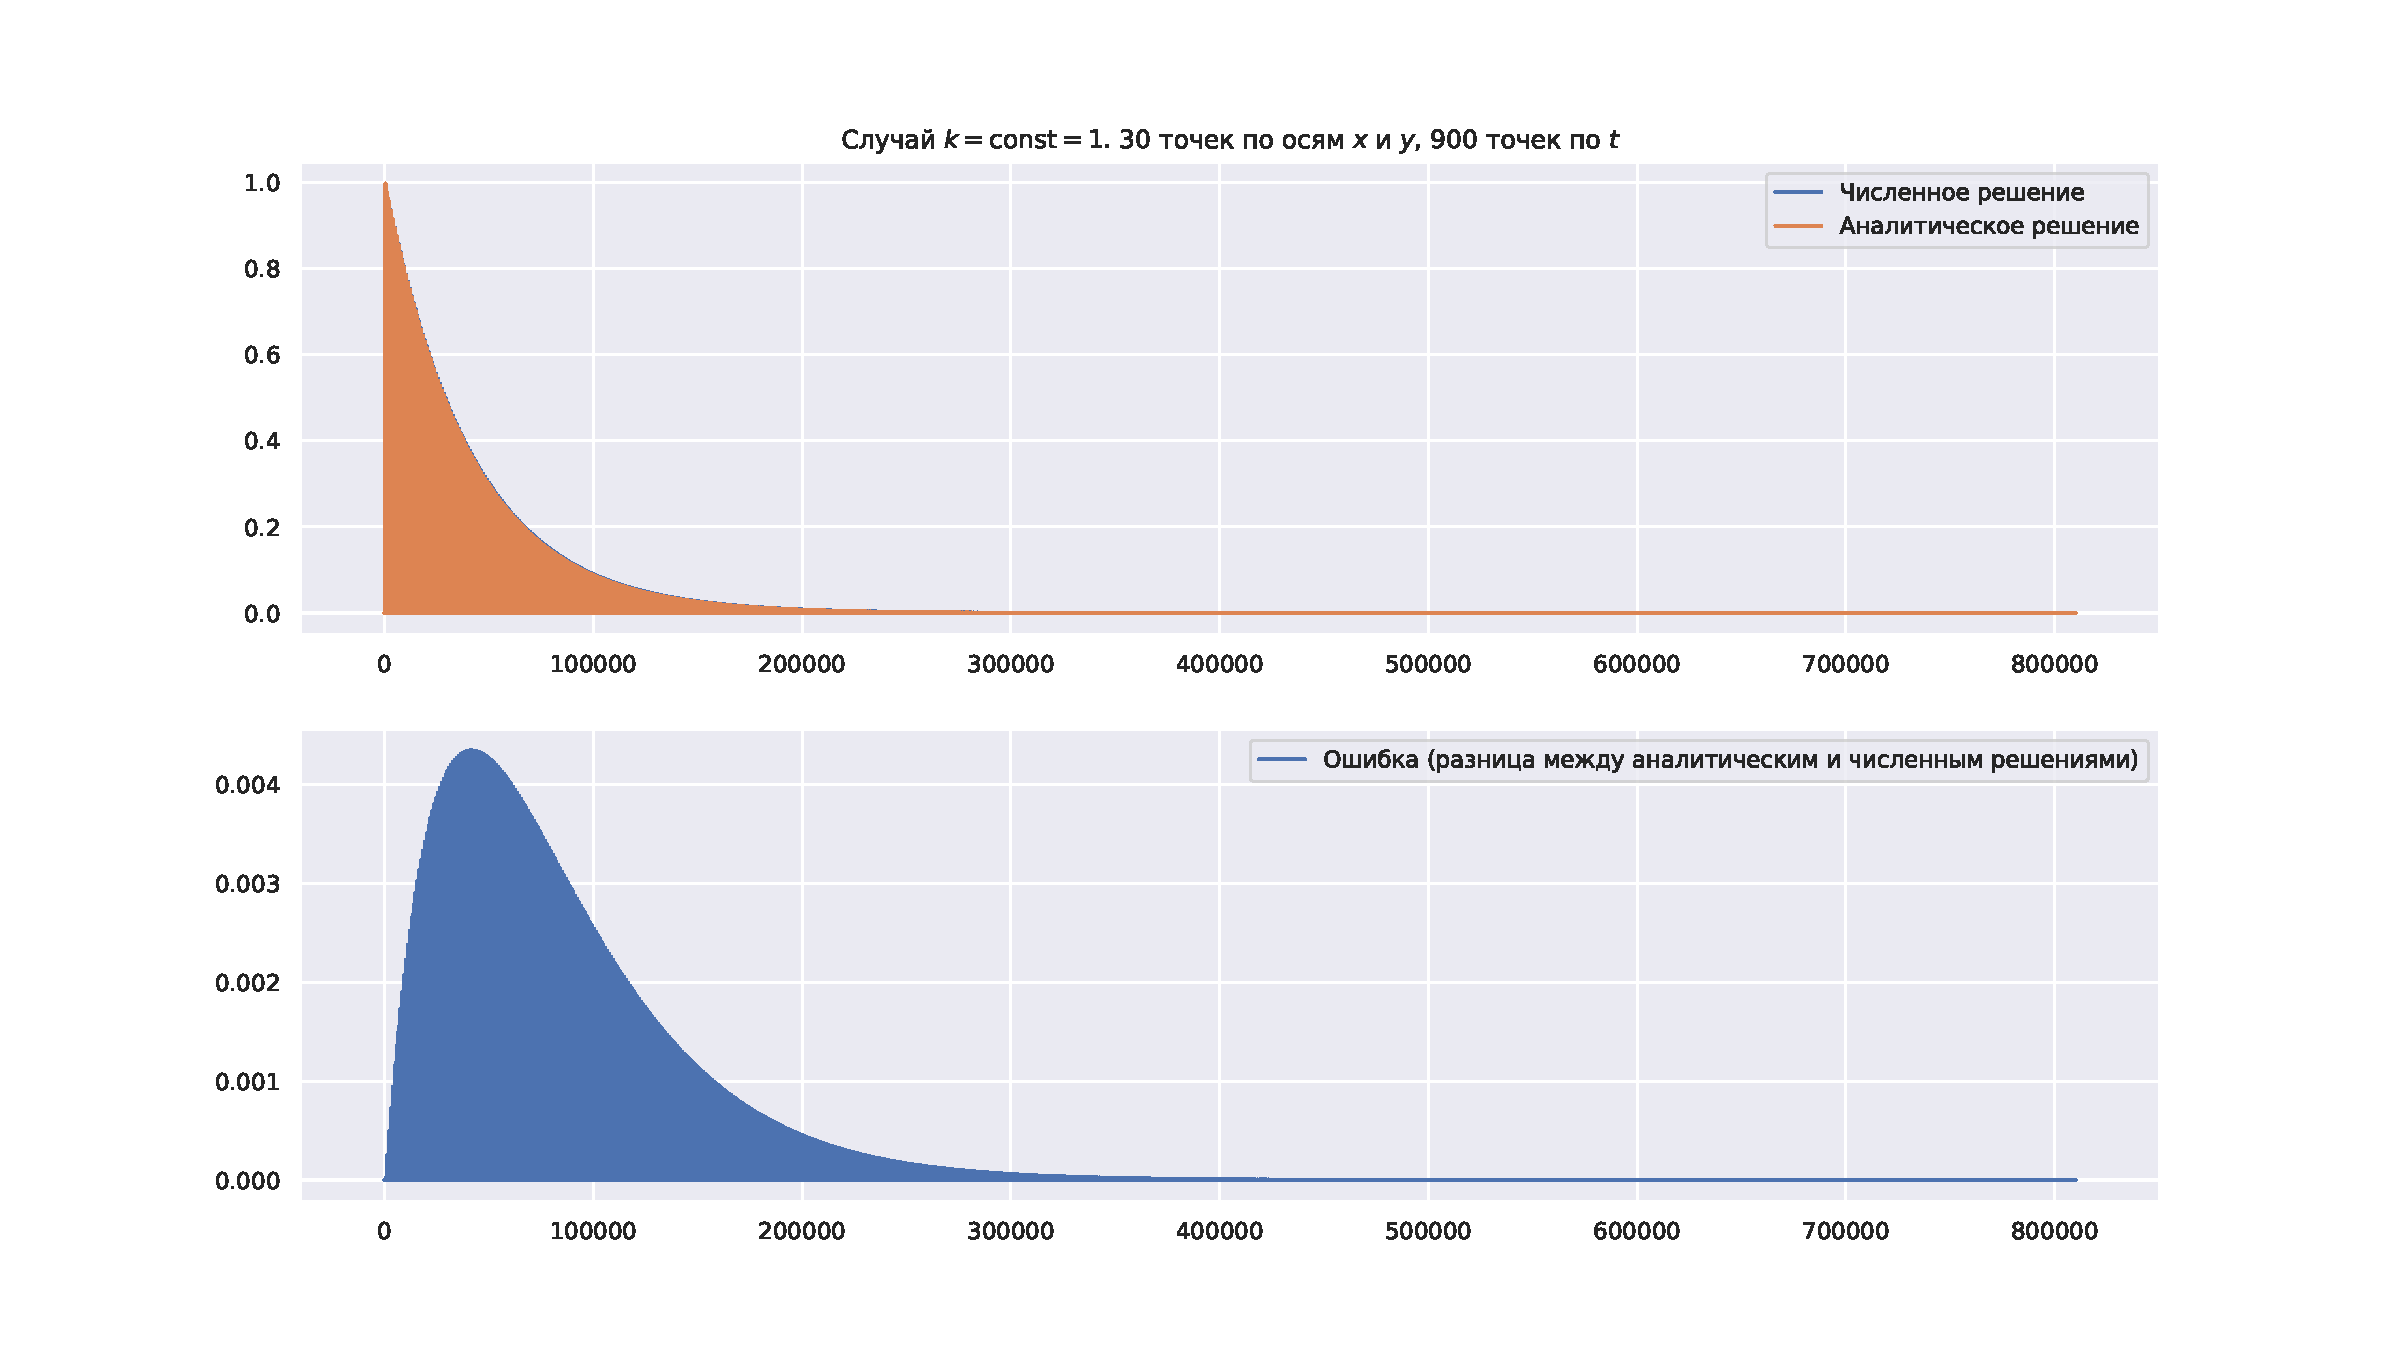
\includegraphics[scale=0.44]{figs/constantksol.pdf}
    \caption{Замыкание на постоянный $k$.}
    \label{constk}
\end{figure}

\subsection{Непостоянный $k$}
Рассмотрим $k(x,y) \neq \text{const}$:
\begin{equation*} 
    u_t(t, x) = \operatorname{div} (k(x,y) \operatorname{grad} u(t, x)) = u_x + x(u_{xx}+u_{yy}).
\end{equation*}
Если рассмотреть краевое условие:
\begin{align*} 
    &u(t, x, y) \big| _{x \in \partial \Omega} = 0, \quad \Omega = [0,1]\times [0,1]. \\
    &u(0, x, y) = e^x \sin y, \quad x \in \Omega. 
\end{align*}
То можно (мне повезло) угадать решение:
$$
u(t, x, y) = e^t e^x \sin y.
$$
 \end{document}